\documentclass[newPxFont,numfooter,sectionpages]{beamer}
\usepackage[utf8]{inputenc}
\usepackage{hyperref}
\hypersetup{colorlinks=true, urlcolor=blue}
\usetheme{sthlm}
\usepackage{pgfplots}
\pgfplotsset{compat=1.14}
\usepackage{cancel}

%-=-=-=-=-=-=-=-=-=-=-=-=-=-=-=-=-=-=-=-=-=-=-=-=
%
%	PRESENTATION INFORMATION
%
%-=-=-=-=-=-=-=-=-=-=-=-=-=-=-=-=-=-=-=-=-=-=-=-=

\title{Evolutionary epidemiology in the 21st century}
\subtitle{Data integration and modelling strategies}
% \date{\today}
\author{Luiz Max Carvalho}
\institute{}

\hypersetup{
pdfauthor = {LMCarvalho: lm.carvalho@ed.ac.uk},
pdfsubject = {EvoEpi},
pdfkeywords = {Bayesian statistics, phylogenetics, data integration},
pdfmoddate= {D:\pdfdate},
pdfcreator = {}
}

\begin{document}

%-=-=-=-=-=-=-=-=-=-=-=-=-=-=-=-=-=-=-=-=-=-=-=-=
%
%	TITLE PAGE
%
%-=-=-=-=-=-=-=-=-=-=-=-=-=-=-=-=-=-=-=-=-=-=-=-=

\maketitle

%-=-=-=-=-=-=-=-=-=-=-=-=-=-=-=-=-=-=-=-=-=-=-=-=
%	FRAME: Acks
%-=-=-=-=-=-=-=-=-=-=-=-=-=-=-=-=-=-=-=-=-=-=-=-=
\begin{frame}{Acknowledgements}
\begin{columns}
\begin{column}{0.3\textwidth}
    \begin{figure}
     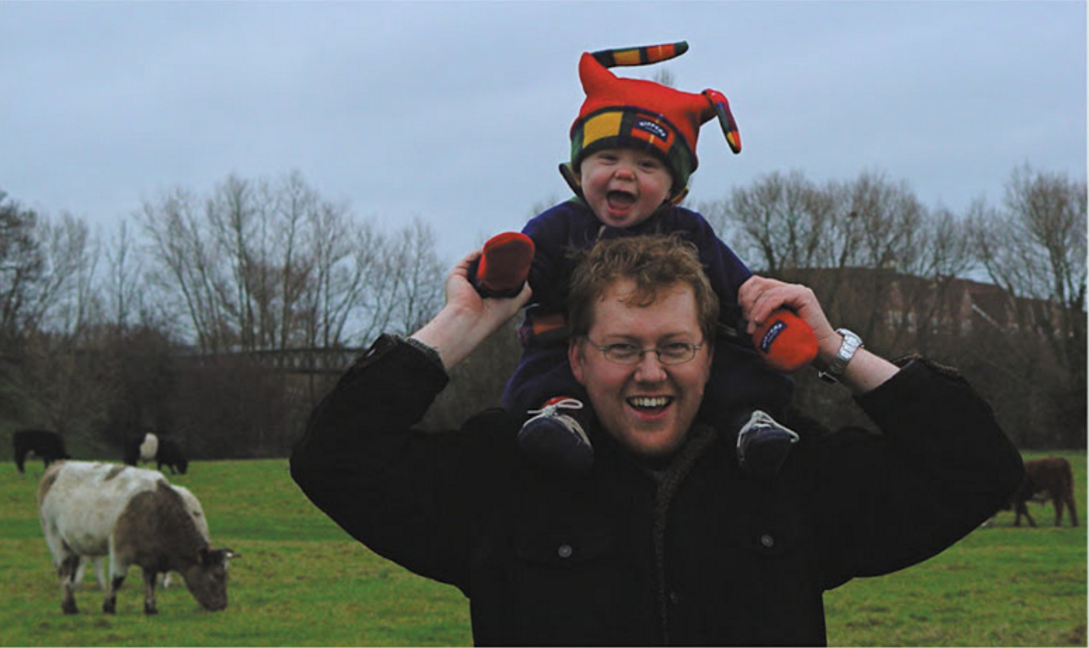
\includegraphics[width=\textwidth]{figures/rambaut.png} \\
     Andrew Rambaut \\
     University of Edinburgh
     \end{figure}
\end{column}
\begin{column}{0.3\textwidth}  %%<--- here
    \begin{figure}
     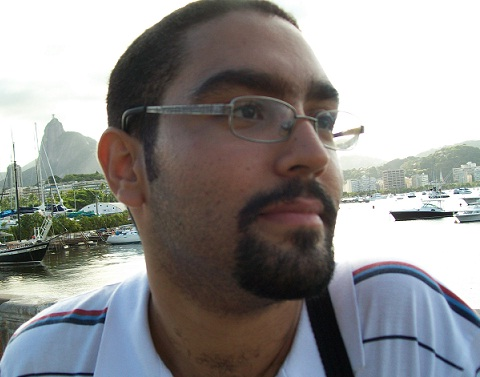
\includegraphics[width=\textwidth]{figures/leonardobacelarlimasantos.jpg}\\
     Leo Santos\\
     CEMADEN
     \end{figure}
\end{column}
% \begin{column}{0.3\textwidth}  %%<--- here
%     \begin{figure}
%      \includegraphics[width=\textwidth]{figures/baele.png} \\
%      Guy Baele \\
%      KU Leuven
%      \end{figure}
% \end{column}
\end{columns}
\end{frame}

%-=-=-=-=-=-=-=-=-=-=-=-=-=-=-=-=-=-=-=-=-=-=-=-=
%	FRAME: Nice to meet
%-=-=-=-=-=-=-=-=-=-=-=-=-=-=-=-=-=-=-=-=-=-=-=-=
\begin{frame}{Who's this guy?}
\begin{itemize}
\item Have a degree in Biology, can't tell an insect from a spider;
\item PhD student in Evolutionary Biology (!) at the University of Edinburgh;
\item Work mainly in \textbf{Quantitative Biology};
\item Interests include \textbf{Markov chain Monte Carlo}, \textbf{complex networks} and \textbf{risk modelling}. 
\end{itemize}
\end{frame}

%-=-=-=-=-=-=-=-=-=-=-=-=-=-=-=-=-=-=-=-=-=-=-=-=
%	FRAME: Outline
%-=-=-=-=-=-=-=-=-=-=-=-=-=-=-=-=-=-=-=-=-=-=-=-=
\begin{frame}{Outline}
\begin{alertblock}{Evolutionary epidemiology}
Concepts and tools.
\end{alertblock}\pause
\begin{exampleblock}{Challenges and opportunities}
Methodological issues, data collection and handling.
\end{exampleblock}\pause
\begin{block}{The role of mathematics}
Which areas of mathematics are more heavily involved.
\end{block}\pause
\begingroup
\setbeamercolor{block title}{fg=white, bg=\cnPurple}
\setbeamercolor{block body}{bg=\cnLightPurple}
\begin{block}{Much more work is needed}
We should prepare for an era of plenty.
\end{block}
\endgroup
\end{frame}

%-=-=-=-=-=-=-=-=-=-=-=-=-=-=-=-=-=-=-=-=-=-=-=-=
%	FRAME: Phylodynamics
%-=-=-=-=-=-=-=-=-=-=-=-=-=-=-=-=-=-=-=-=-=-=-=-=
\begingroup
% \setbeamercolor{frametitle}{bg=\cnRed}
% \setbeamercolor{normal text}{fg=\cnDarkGrey,bg=\cnLightRed}
\begin{frame}{Motivation}
\begin{block}{Phylodynamics of fast-evolving viruses}
 Inferring spatial and temporal dynamics from genomic data:
 \begin{center}
  \Large \textbf{Phylogenies}$^\ast$! \\
  \tiny $^\ast$ plus complicated models
 \end{center}
\end{block}
\begin{figure}
	\centerline{
	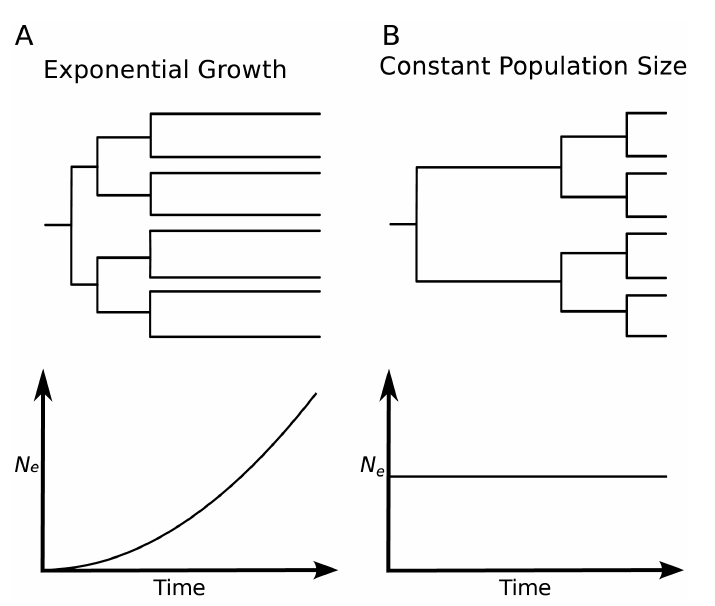
\includegraphics[width=0.5\textwidth,height=5cm]{figures/pop_growth.jpg} \\ 
	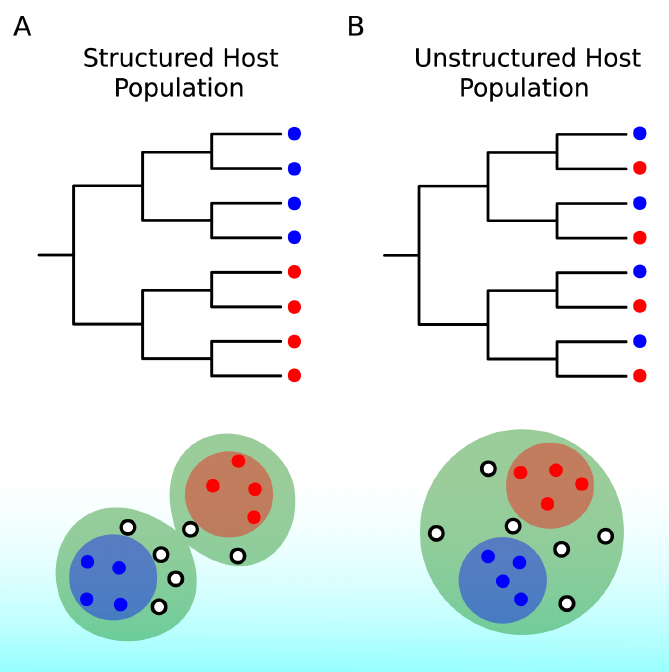
\includegraphics[width=0.5\textwidth,height=5cm]{figures/pop_structure.jpg}
	}
\end{figure}
\end{frame}
\endgroup

%-=-=-=-=-=-=-=-=-=-=-=-=-=-=-=-=-=-=-=-=-=-=-=-=
%	FRAME: 
%-=-=-=-=-=-=-=-=-=-=-=-=-=-=-=-=-=-=-=-=-=-=-=-=
\begin{frame}{Trees and the coalescent}

\begin{column}{0.5\textwidth}
 \begin{figure}[!h]
\begin{center}
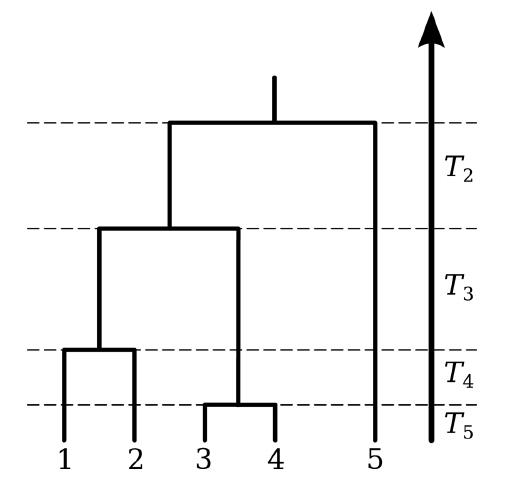
\includegraphics[scale=.45]{figures/coaltimes.jpg}
\caption{Figure 4 from Volz et al. (2013).}
\end{center}
\end{figure}
\end{column}
\begin{column}{0.45\textwidth}
{\tiny
 Let $T_n$ denote the time for $n$ lineages to~\textit{coalesce}, i.e., merge into one ancestral lineage, in a population of size $N_e$.
 Then:
\begin{align*}
Pr(T_n = t) &= \lambda_n e^{-\lambda_nt}\\
\lambda_n &= \binom{n}{2}\frac{1}{N_e} = \binom{n}{2}\frac{1}{N_e\tau}
\end{align*}
where $N_e$ is the effective population size and $\tau$ is the generation time.
Let $T_{\text{mrca}}$ denote the age of the most recent common ancestor:
\begin{align*}
 \mathbb{E}[T_{\text{mrca}}] &= \mathbb{E}[T_n] + \mathbb{E}[T_{n-1}] + \ldots + \mathbb{E}[T_2]\\
 &= 1/\lambda_n + 1/\lambda_{n-1} + \ldots + 1/\lambda_2\\
 &= 2N_e(1-\frac{1}{n})
\end{align*}
}
\end{column}
\end{frame}

%-=-=-=-=-=-=-=-=-=-=-=-=-=-=-=-=-=-=-=-=-=-=-=-=-=-=-=-=
%	FRAME: Data Integration I: Ebola epidemics in West Africa
%-=-=-=-=-=-=-=-=-=-=-=-=-=-=-=-=-=-=-=-=-=-=-=-=-=-=-=-=

\begin{frame}{Data Integration I: Ebola epidemics in West Africa}
\href{http://virological.org/t/phylogeography-of-2014-2015-ebola-virus-epidemic/199}{[animation]}
\begin{figure}
	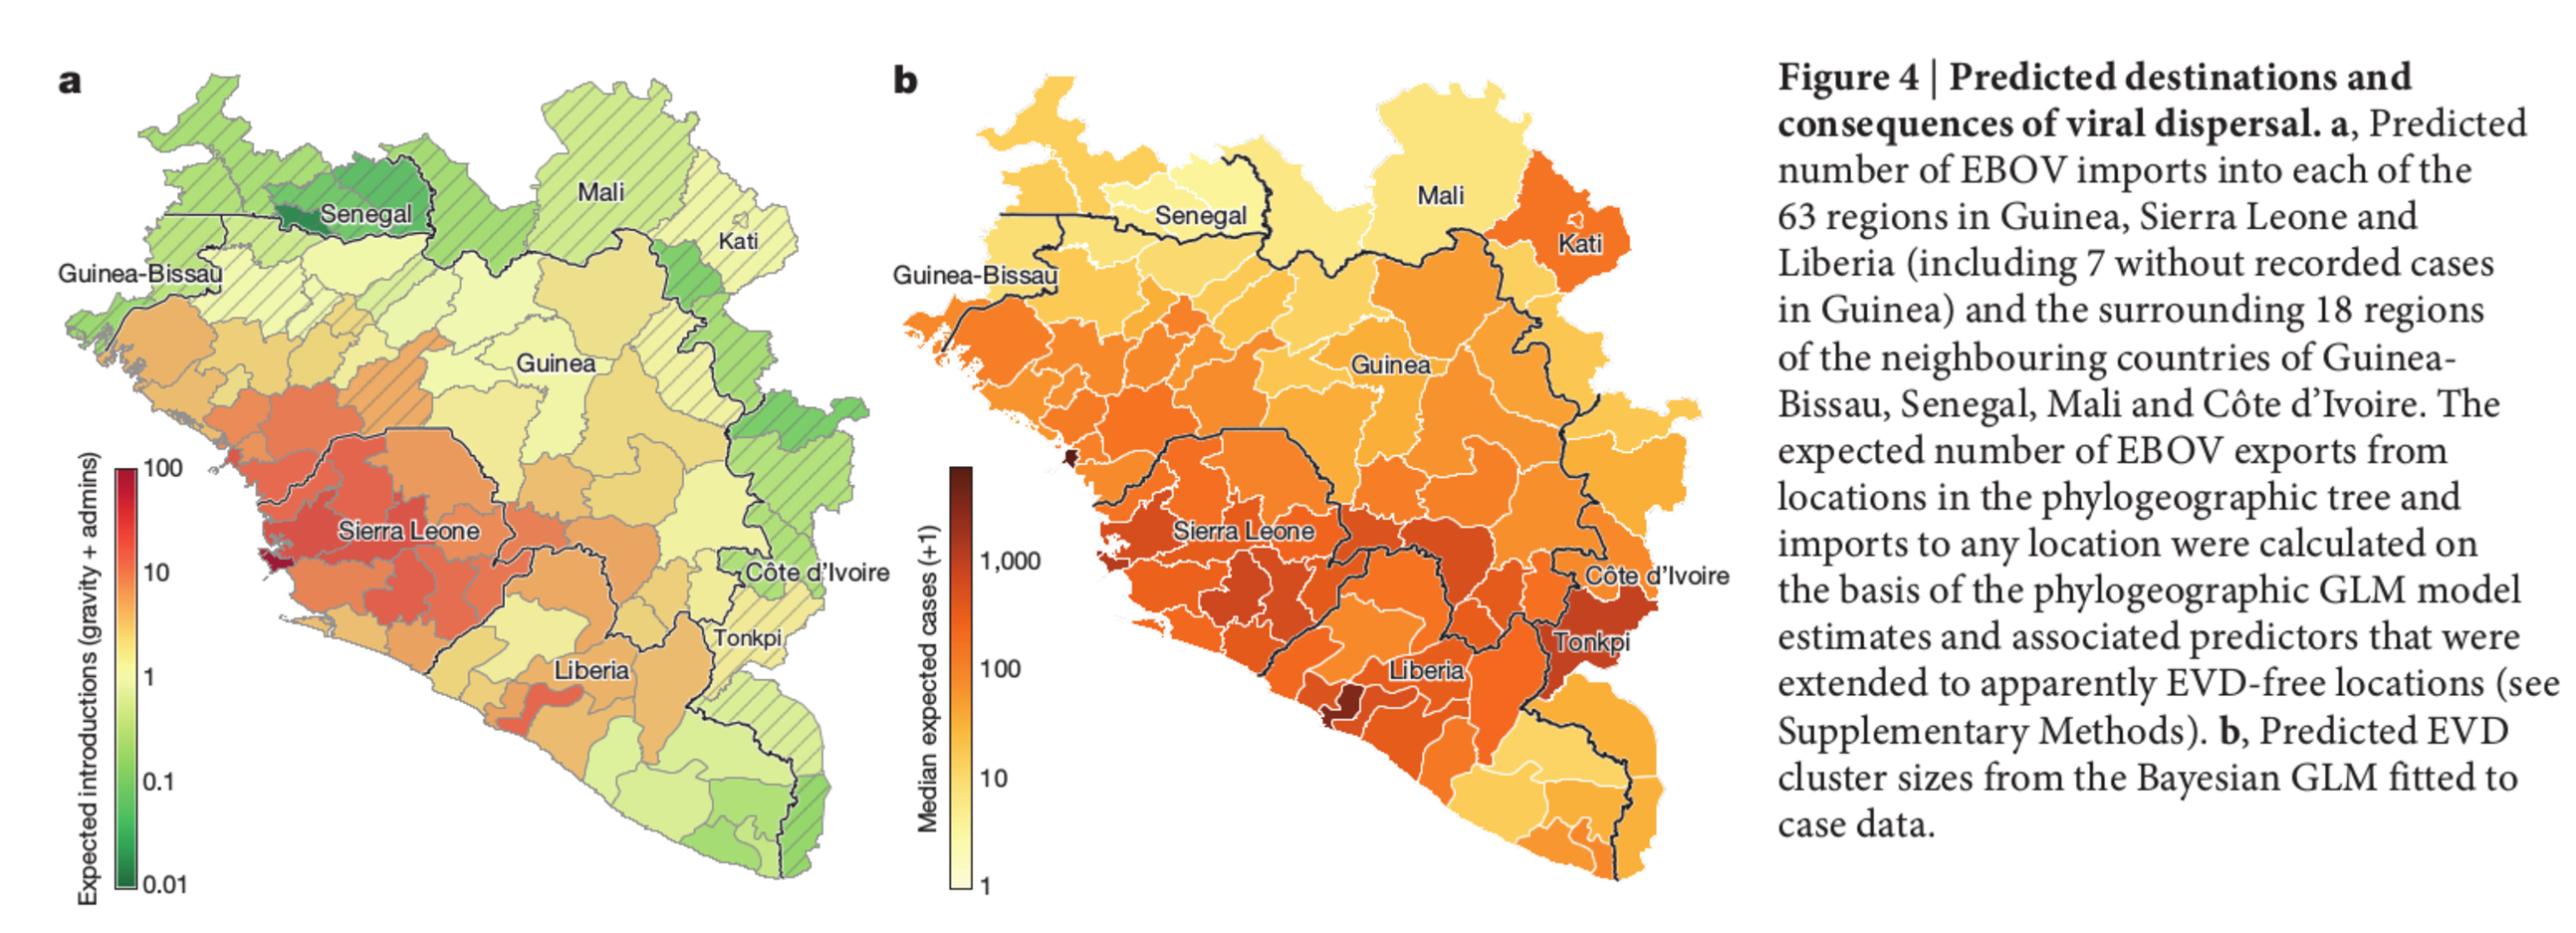
\includegraphics[scale=.30]{figures/ebov_glm_predictions.pdf} 
\end{figure}
\end{frame}

%-=-=-=-=-=-=-=-=-=-=-=-=-=-=-=-=-=-=-=-=-=-=-=-=-=-=-=-=
%	FRAME: Data Integration II: GPA82V mutation in EBOV GP and disease severity
%-=-=-=-=-=-=-=-=-=-=-=-=-=-=-=-=-=-=-=-=-=-=-=-=-=-=-=-=
\begin{frame}{Data Integration II: GPA82V mutation and mortality}
\begin{figure}
	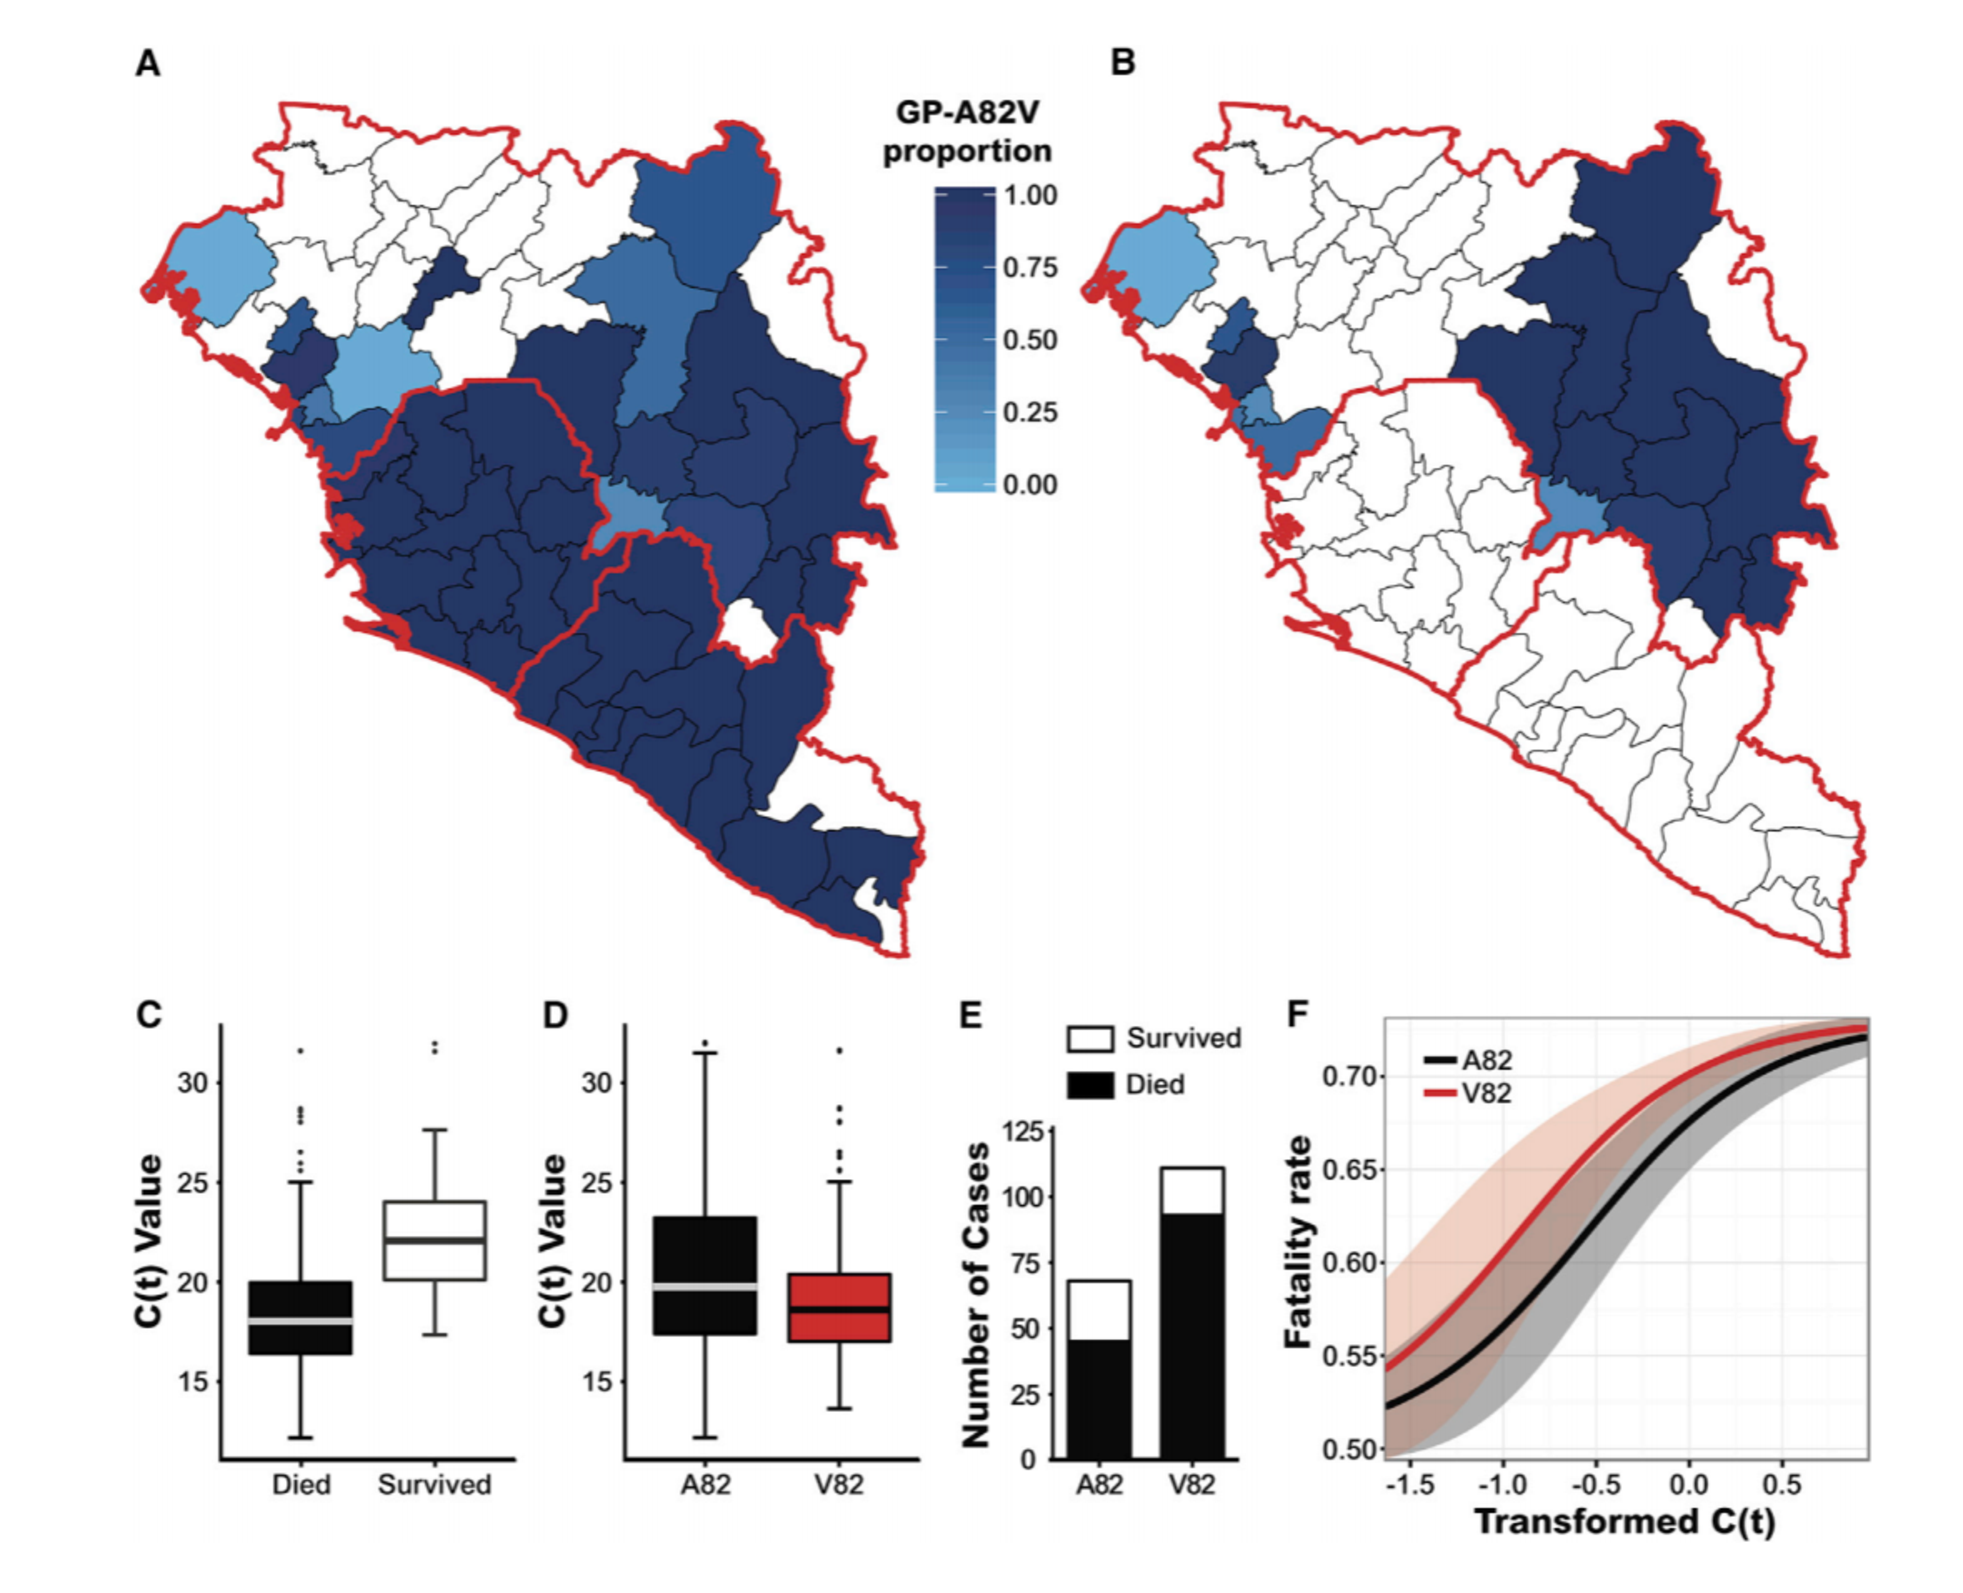
\includegraphics[scale=.30]{figures/gpa82v_results.pdf} 
\end{figure}
\end{frame}

%-=-=-=-=-=-=-=-=-=-=-=-=-=-=-=-=-=-=-=-=-=-=-=-=-=-=-=-=
%	FRAME: Potential applications
%-=-=-=-=-=-=-=-=-=-=-=-=-=-=-=-=-=-=-=-=-=-=-=-=-=-=-=-=
\begin{frame}{Potential applications}
\begin{itemize}
 \item Human mobility + case data = epidemiological models of spread and maintenance;
 \item Genomic data + environmental data = predictions of flow and case counts (e.g. Leptospirosis).
 
\end{itemize}
\begin{figure}
	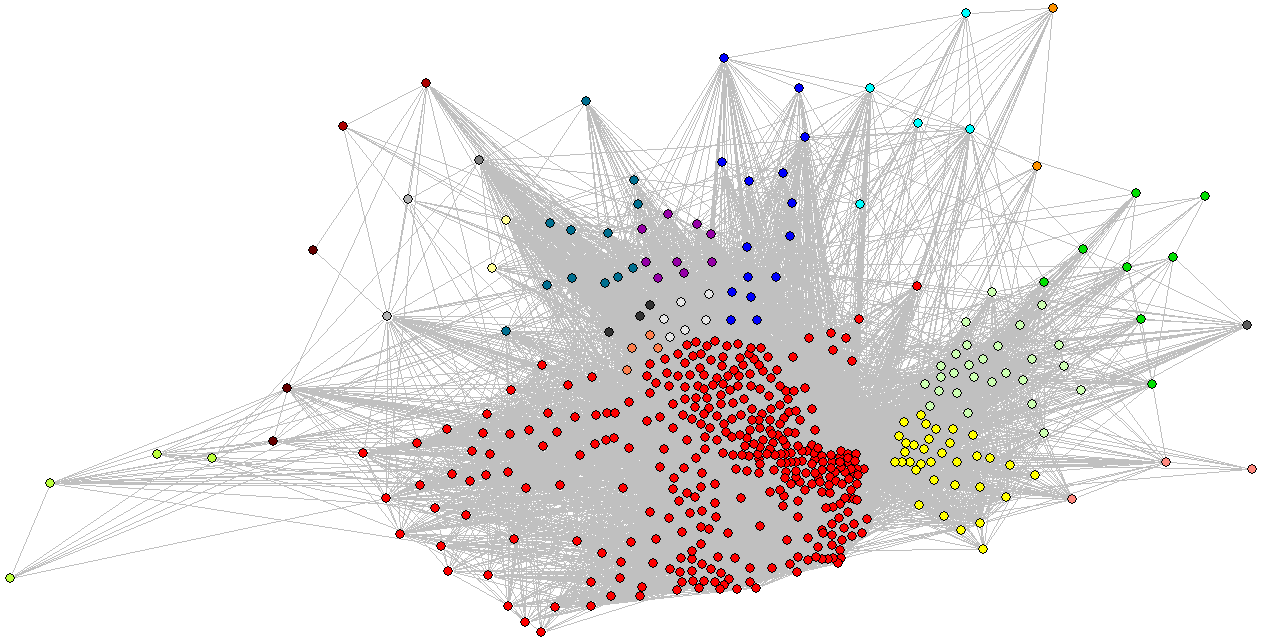
\includegraphics[scale=.30]{figures/mobility_network.png} 
\end{figure}
\end{frame}

% -=-=-=-=-=-=-=-=-=-=-=-=-=-=-=-=-=-=-=-=-=-=-=-=
% 	FRAME: Mathematics involved
% -=-=-=-=-=-=-=-=-=-=-=-=-=-=-=-=-=-=-=-=-=-=-=-=
% \begin{frame}{What about the Maths?}
% \begin{itemize}
%  \item \textbf{Graph Theory}: trees are planar graphs.
%  \item \textbf{Combinatorics}: trees are discrete objects, loads of combinatorial arguments
%  \item \textbf{Stochastic processes}: inference from aligned DNA sequences relies heavily on Markov chain theory, Brownian motion and more.
% 
% \end{itemize}
% 
% \end{frame}

%-=-=-=-=-=-=-=-=-=-=-=-=-=-=-=-=-=-=-=-=-=-=-=-=
%	FRAME: Take home
%-=-=-=-=-=-=-=-=-=-=-=-=-=-=-=-=-=-=-=-=-=-=-=-=
\begin{frame}{Take home}
\begin{exampleblock}{Phylodynamics is a powerful tool}
DNA sequences from pathogens + environmental/socio-economic data can give us insight
\end{exampleblock}\pause
\begin{alertblock}{Searching trees is \textbf{hard}}
Developing better statistical models and computational tools is crucial.
\end{alertblock}\pause
\begin{block}{Data integration is crucial}
 We need more and better data.
\end{block}\pause
\begingroup
\setbeamercolor{block title}{fg=white, bg=\cnPurple}
\setbeamercolor{block body}{bg=\cnLightPurple}
\begin{block}{Nature is complicated}
We need better models to go along.
\end{block}
\endgroup
\end{frame}

%-=-=-=-=-=-=-=-=-=-=-=-=-=-=-=-=-=-=-=-=-=-=-=-=
%	FRAME: bye bye
%-=-=-=-=-=-=-=-=-=-=-=-=-=-=-=-=-=-=-=-=-=-=-=-=
\begingroup
\setbeamercolor{background canvas}{bg=\cnDarkGrey}
\begin{frame}[plain]

\centering{\cGrey{\Huge{THE \newline END}}}

\end{frame}
\endgroup

\end{document}